\section{Preliminaries}\label{SectPreliminaries}
We recall basic facts about the quantum groups $\Oq$ and $\Uq$, and the needed constructions and properties of skein categories in~\cite{Cooke} and of stated skein algebras in \cite{Cos}. We finish with a slight modification of the construction of internal skein algebras of \cite{Gunningham}. Let $k$ be either $\mathbb{Q}\big(q^{\frac{1}{2}}\big)$ or $\mathbb{C}$ with $q^{\frac{1}{2}} \in \mathbb{C}^\times$ generic, i.e., not a root of unity. We work in the symmetric monoidal (2,1)-category ${\rm Cat}_k$ of small $k$-linear categories, $k$-linear functors and natural isomorphisms, where the tensor product $\mathcal{C} \otimes \mathcal{D}$ has objects $\operatorname{Ob}(\mathcal{C}) \times \operatorname{Ob}(\mathcal{D})$ and morphisms $\Hom_{\mathcal{C} \otimes \mathcal{D}}((c,d),(c',d')) := \Hom_\mathcal{C}(c,c') \otimes_k \Hom_\mathcal{D}(d,d')$.

\subsection[The coribbon Hopf algebra O\_\{q\textasciicircum{}2\}(SL\_2)]
{The coribbon Hopf algebra $\boldsymbol{\Oq}$}\label{SectRibCat}

We recall the definition of the coribbon Hopf algebra $\Oq$, its categories of right comodules and their links with left $\Uq$-modules.
\begin{Definition}
The coribbon Hopf algebra $\Oq$ is the free $k$-algebra with
(one should read the matrix equations component-wise, and the tensor product of matrices should be computed as a usual matrix product with tensor products of coefficients instead of products)
\begin{alignat*}{3}
& \text{generators}\colon&& a,\ b,\ c,\ d,&
\\
& \text{relations}\colon&& ca = q^2ac,\quad db = q^2bd,\quad ba = q^2ab,\quad dc = q^2cd,&
\\
&&& bc = cb,\quad ad - q^{-2}bc = 1\quad \text{and}\quad da - q^2cb = 1,&
\\
&\text{coproduct}\colon&&\Delta\begin{pmatrix} a & b \\[-.5ex] c & d \end{pmatrix}
= \begin{pmatrix} a & b \\[-.5ex] c & d \end{pmatrix} \otimes \begin{pmatrix} a & b \\[-.5ex] c & d \end{pmatrix}\!,&
\\
& \text{counit}\colon&& \varepsilon \begin{pmatrix} a & b \\[-.5ex] c & d \end{pmatrix}
= \begin{pmatrix} 1& 0 \\[-.5ex] 0 & 1\end{pmatrix}\!,&
\\
& \text{antipode}\colon&& S \begin{pmatrix} a & b \\[-.5ex] c & d \end{pmatrix}
= \begin{pmatrix} d & -q^2b \\[-.5ex] -q^{-2}c & a \end{pmatrix}\!,&
\\
&\text{co-}R\text{-matrix}\colon&& R \begin{pmatrix}
a \otimes a & a \otimes b & b \otimes a & b \otimes b
\\
a \otimes c & a \otimes d & b \otimes c & b\otimes d\\ c\otimes a & c\otimes b & d \otimes a & d\otimes b\\ c\otimes c & b\otimes d & d\otimes c & d\otimes d \end{pmatrix}
=\begin{pmatrix} q& 0 & 0 & 0\\ 0 & q^{-1} & q-q^{-3} & 0\\ 0 & 0 & q^{-1}&0\\ 0 & 0 & 0 & q \end{pmatrix}\!,&
\\
& \text{coribbon functional}\colon \quad && \theta \begin{pmatrix} a & b \\[-.5ex] c & d \end{pmatrix}
= \begin{pmatrix} -q^3 & 0 \\[-.5ex] 0 & -q^3 \end{pmatrix}\!.&
\end{alignat*}
\end{Definition}

\begin{Remark}
We took the coribbon functional so that the twist on a comodule $V$ is given by $\theta_V\colon V \overset{\Delta_V}{\to} V \otimes H \overset{{\rm Id}_V \otimes \theta}{\to} V$. In the literature (see \cite{Wakui} for the coribbon case, or \cite{Kassel} for the ribbon case), the coribbon functional is defined to be $\theta^{-1}$ in our definition.
Moreover, we use here an unusual coribbon functional, which arises naturally on the stated skein algebra of the bigon in Section~\ref{SectStatedSkein}. It is studied in \cite{Tingley} where the author proves that it gives precisely the Kauffman-bracket relation under the Reshetikhin--Turaev functor, whereas the usual coribbon functional gives relations which differ by a sign, and give the Jones polynomial after writhe renormalisation.\looseness=-1
\end{Remark}

\begin{Definition}\label{defOqcomods}
The quantum plane $\mathbb{A}_{q^2}^2$ is the free $k$-algebra generated by $x$ and $y$ modulo the relation $yx = q^2xy$. It is a right $\Oq$-comodule algebra with $\Delta \left(\begin{smallmatrix} x&y \end{smallmatrix}\right) = \left(\begin{smallmatrix} x&y \end{smallmatrix}\right) \otimes \left( \begin{smallmatrix} a & b \\ c & d \end{smallmatrix}\right)$ on generators.

Its subspace of homogeneous polynomials of degree $n$ forms a sub-comodule which we denote by~$V_n$.
In particular the generators span the comodule $V_1$ which we abbreviate $V$ and call the standard co-representation of $\Oq$. It is more conventional to call its basis $v_+ = x$ and $v_- = y$. This comodule is self dual. The left dual $V^*$ of $V$ has basis $v_+^*$ and $v_-^*$, and one has an isomorphism of $\Oq\text{-comodules}$
\begin{gather*}
\varphi \colon \
\begin{cases}
V \to V^*,
\\
v_+ \mapsto -q^{\frac{5}{2}} v_-^*,
\\[.5ex]
v_- \mapsto q^{\frac{1}{2}}v_+^*.
\end{cases}
\end{gather*}
\end{Definition}

{\sloppy\begin{Proposition}[{\cite[Section~4.2.1]{Klimyk}}]\label{propOqSemiSimple}
The $\Oq$-comodules $V_n,\ n \in \mathbb{N}$, are all the simple $\Oq$-comodules. Moreover, the categories $\Oq\text{-}{\rm comod}$ and $\Oq\text{-}{\rm comod}^{\rm fin}$ are semi-simple.
\end{Proposition}}

\begin{Definition}
The Hopf algebra $\Uq$ is the free $k$-algebra with:
\begin{alignat*}{3}
& \text{generators}\colon\quad  &&E,\,F,\,K,&
\\
&\text{relations}\colon && KE=q^4EK, \quad KF=q^{-4}FK,\quad  EF-FE = \frac{K-K^{-1}}{q^2-q^{-2}},&
\\
&\text{coproduct}\colon &&\Delta (K) = K \otimes K,\quad \Delta (E) = 1\otimes E+E\otimes K,\quad \Delta (F) = K^{-1}\otimes F + F\otimes 1,&
\\
& \text{counit}\colon && \varepsilon(K)=1,\quad\varepsilon(E)=\varepsilon(F)=0,&
\\
& \text{antipode}\colon && S(K) = K^{-1},\quad S(E) = -EK^{-1},\quad S(F) =-KF.&
\end{alignat*}
\end{Definition}

\begin{Definition}
The left $\Uq$-module $V_{\pm,n}$ is the vector space of dimension $n+1$ with action:
\begin{gather*}
 K=\pm \setlength{\arraycolsep}{1.5pt}\begin{pmatrix}
 q^{2n} & 0& \cdots & 0 \\ 0& q^{2(n-2)} &\ddots &\vdots \\ \vdots &\ddots &\ddots&0 \\ 0 &\cdots&0& q^{-2n}\end{pmatrix}\!,\qquad
 E=\setlength{\arraycolsep}{2.5pt}\begin{pmatrix}
 0 & [n]_{q^2}& & 0 \\ & \ddots &\ddots & \\ \vdots & &\ddots&[1]_{q^2} \\ 0 & \cdots & & 0\end{pmatrix}\!,\\
 F=\setlength{\arraycolsep}{2.5pt}\pm \begin{pmatrix}
 0 & & \cdots & 0 \\ {[1]_{q^2}} & \ddots & & \vdots\\ & \ddots&\ddots& \\ 0 & & [n]_{q^2}& 0\end{pmatrix}\!,
 \end{gather*}
 where $ [n]_{q^2} = \frac{q^{2n}-q^{-2n}}{q^2-q^{-2}}$.

The modules of the form $V_{+,n}$ are called of type 1, and the others are discarded here. The mo\-du\-le~$V_{+,1}$ is denoted by $V$ and called the standard representation of $\Uq$.
A module $W$ is called locally finite (of type 1) if $\forall w \in W$, $\Uq \cdot w$ is finite-dimensional (and isomorphic to some $V_{+,n}$).
\end{Definition}

\begin{Proposition}[{\cite[Theorem~VII.2.2]{Kassel}}]
The $\Uq$-modules $V_{\pm,n},\ n \in \mathbb{N}$ are all the locally finite simple $\Uq$-modules. Moreover, the categories $\Uq\text{-}{\rm mod}^{\rm lf}$ and $\Uq\text{-}{\rm mod}^{\rm fin}$, of respectively locally finite and finite-dimensional $\Uq$-modules of type $1$, are semi-simple.
\end{Proposition}

\begin{Definition}
We can define a dual pairing, namely a non-degenerate bilinear form
\[
\langle \cdot,\cdot\rangle \colon \  \Uq \otimes \Oq \to k
\] satisfying $\langle x, y.y'\rangle = \langle x_{(1)},y\rangle \langle x_{(2)},y'\rangle$, $\langle x.x', y\rangle = \langle x,y_{(1)}\rangle \langle x',y_{(2)}\rangle$, $\langle x,1\rangle = \varepsilon(x)$, $\langle 1,y\rangle = \varepsilon(y)$ and $\langle S(x),y\rangle = \langle x,S(y)\rangle$. It is given on generators by
\begin{gather*}
 \left\langle K,\begin{pmatrix}a&b\\c&d \end{pmatrix} \right\rangle =
 \begin{pmatrix}q^2&0\\0&q^{-2} \end{pmatrix}\!, \qquad \!
 \left\langle E,
 \begin{pmatrix}a&b\\c&d \end{pmatrix} \right\rangle =
 \begin{pmatrix}0&1\\0&0 \end{pmatrix}\!,\qquad \!
 \left\langle F,\begin{pmatrix} a&b\\c&d \end{pmatrix}\right\rangle =
 \begin{pmatrix}0&0\\1&0 \end{pmatrix}\!.
 \end{gather*}
 A right $\Oq$-comodule structure on some vector space $W$ induces a left $\Uq$-module structure by $x\cdot w = w_{(1)}. \langle x,w_{(2)} \rangle$, $x \in \Uq$, $w\in W$.
\end{Definition}

\begin{Proposition}[{\cite[equation~(3.3), p.~126]{Abe}, \cite[Theorem~7.9]{Takeuchi}}]\label{propOqcomodUqmod}
This correspondence induces equivalences of categories $\Oq\text{-}{\rm comod}^{\rm fin}\simeq \Uq\text{-}{\rm mod}^{\rm fin}$ and $\Oq\text{-}{\rm comod} \simeq \Uq\text{-}{\rm mod}^{\rm lf}$.

The simple comodules $V_n$ are mapped on the simple modules $V_{+,n}$.
\end{Proposition}

Note that this correspondence also preserves the monoidal (and actually ribbon, though using an unusual twist on $\Uqmod$) structure. In the following, we will mostly adopt the point of view of comodules over $\Oq$, because there are fewer conditions to ask, the braided and ribbon structure of $\Oq$ is algebraic and not ``topological'', and it has a geometric description using stated skein algebras.


\subsection{Skein categories}\label{SectSkCat}
Tangle invariants obtained from a $k$-linear ribbon category $\mathcal{V}$ are defined in \cite[Section~I.2]{Turaev}. They can be extended to give tangle invariants on any oriented surface $\Sigma$ by local relations, and produce the skein category of the surface ${\rm Sk}_\mathcal{V}(\Sigma)$, see \cite{Walker}. We will use and recall their boundary structure and excision properties, see \cite{Cooke}.

\begin{Definition}
Let $[n]$ denote the set of $n$ points $\{1,\ldots,n\} \times \{0\}$ in $\mathbb{R}^2$, equipped with blackboard framing (coming out of the page when we draw ribbon graphs as below) and ${\rm Ribbon}_\mathcal{V}$ the category whose objects are framed oriented $\mathcal{V}$-coloured points of $\mathbb{R}^2$ of the form $[n]$, and morphisms ribbon graphs (i.e., $\mathcal{V}$-coloured oriented framed tangles with coupons coloured by morphisms) between them in $\mathbb{R}^2\times[0,1]$.
\end{Definition}
$$
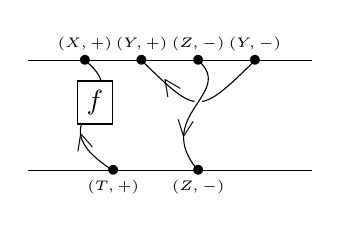
\begin{tikzpicture}[baseline = 15pt, yscale = 0.7, xscale = 1.2]
\draw (0,2) -- (3,2) node[pos = 0.2]{\small $\bullet$} node[pos = 0.2, above]{\tiny $(X,+)$} node[pos = 0.4]{\small $\bullet$} node[pos = 0.4, above]{\tiny $(Y,+)$} node[pos = 0.6]{\small $\bullet$} node[pos = 0.6, above]{\tiny $(Z,-)$} node[pos = 0.8]{\small $\bullet$} node[pos = 0.8, above]{\tiny $(Y,-)$};
\draw (0,0) -- (3,0) node[pos = 0.3]{\small $\bullet$} node[pos = 0.3, below]{\tiny $(T,+)$} node[pos = 0.6]{\small $\bullet$} node[pos = 0.6, below]{\tiny $(Z,-)$};
\draw (0.9,0) .. controls (0,1) and (1.2,1.2) .. (0.6,2) node[pos=0.2, sloped]{$<$} node [pos = 0.6, rectangle, draw, fill=white]{$f$};
\draw (1.2,2) .. controls (1.8,1) .. (2.4,2) node[fill, color= white, midway, circle, scale = 0.3]{} node[pos = 0.2, sloped]{$<$};
\draw (1.8,0) .. controls (1.3,1) and (2.2,1.4) .. (1.8,2) node[pos = 0.3, sloped]{$<$};
\end{tikzpicture}
$$

\begin{Theorem}[Reshetikhin--Turaev]\label{thmturaev} Given $\mathcal{V}$ a strict ribbon category, there exists a unique strictly monoidal functor ${\rm RT}\colon {\rm Ribbon}_\mathcal{V} \to \mathcal{V}$, called the Reshetikhin--Turaev functor, mapping positive single points to their colour, preserving ribbon structures and mapping coupons to their colour.
\end{Theorem}

\begin{Remark}\label{rmkEqCatSkR2VV}
For skein categories, we would prefer to consider all points with all possible framings instead of only those of the form $[n]$ as in ${\rm Ribbon}_\mathcal{V}$. We denote this bigger category by ${\rm Ribbon}_\mathcal{V}\big(\mathbb{R}^2\big)$. The two categories are equivalent as the inclusion of the first in the second is obviously fully faithful and essentially surjective. A quasi-inverse is however not so natural to define. One has to choose an isomorphism from each object of ${\rm Ribbon}_\mathcal{V}\big(\mathbb{R}^2\big)$ to one of the form~$[n]$. This can be done for example by giving lexicographical order on $\mathbb{R}^2$ and pushing all points in good position while preserving this order, then turning the framing clockwise until it is vertical.

Working with ${\rm Ribbon}_\mathcal{V}\big(\mathbb{R}^2\big)$, and allowing non-strict ribbon categories $\mathcal{V}$, the above theorem still holds, but the functor ${\rm RT}$ is only essentially unique. We now assume a choice of quasi-inverse as above has been made, so that the functor ${\rm RT}$ is defined on ${\rm Ribbon}_\mathcal{V}\big(\mathbb{R}^2\big)$.
\end{Remark}

The above functor ${\rm RT}$ describes a way to obtain invariants of coloured tangles, and actually coloured ribbon graphs, from a ribbon category $\mathcal{V}$. We want to study this invariant, and say that two ribbon graphs are identified if they give the same invariant, namely the same morphism in~$\mathcal{V}$ after evaluation under~${\rm RT}$. Skein categories generalize this construction for coloured ribbon graphs on a thickened surface. The idea is to take the relations between ribbon graph which are true locally, on an embedded cube.

\begin{Definition}
Let $\Sigma$ be a compact oriented surface possibly with boundary and $\mathcal{V}$ a ribbon category. The $k$-linear category ${\rm Ribbon}_\mathcal{V}(\Sigma)$ has objects finite sets of $\mathcal{V}$-coloured oriented framed points of $\Sigma$ and morphisms $k$-linear combinations of isotopy classes of ribbon graphs.

The skein category ${\rm Sk}_\mathcal{V}(\Sigma)$ with coefficients in $\mathcal{V}$ is the quotient of ${\rm Ribbon}_\mathcal{V}(\Sigma)$ by the local relation $\sum \lambda_i F_i = 0$ if there exists an orientation preserving embedding of a cube $\phi\colon [0,1]^3 \hookrightarrow \Sigma \times [0,1]$ such that all of the $F_i$'s coincide outside this little cube, intersect $\phi\big(\partial [0,1]^3\big)$ on either the top or the bottom face, transversally, and give the zero morphism in $\mathcal{V}$ after evaluation of the functor ${\rm RT}$ on this little cube, namely $\sum \lambda_i \mathop{\rm RT}\big(\phi^{-1}(F_i\vert_{{\rm im}\ \phi})\big) = 0$.

Put differently, let $F$ be a ribbon graph and $\phi$ a little cube of $\Sigma \times (0,1)$ such that $G := F\vert_{{\rm im}\ \phi}$ is a (possibly complicated) ribbon graph. Then $\mathop{\rm RT}(G)$ is a morphism in $\mathcal{V}$, and we allow ourselves to replace $G$ with a single coupon coloured by this morphism.
\end{Definition}

\begin{Remark}\label{rmkInclVtoSkMonoid}
When $\Sigma = \mathbb{R}^2$, since ${\rm RT}$ is full, via coupons, it induces an equivalence of categories ${\rm Sk}_\mathcal{V}\big(\mathbb{R}^2\big)\to \mathcal{V}$. Its quasi-inverse is given by the inclusion of the full subcategory $\mathcal{V} \subseteq {\rm Sk}_\mathcal{V}\big(\mathbb{R}^2\big)$ mapping an object $V \in \mathcal{V}$ to the framed point [1] coloured by $V$, and a morphism to a coupon coloured by this morphism.

Note that this inclusion is monoidal but not strictly monoidal, namely one has an isomorphism from the two framed points [2] respectively coloured by $V$ and $W$ to the framed point [1] coloured by $V \otimes W$, this isomorphism is the coupon ${\rm Id}_{V \otimes W}$ with two incoming strands coloured respectively by $V$ and $W$ and one outgoing strand coloured by $V \otimes W$.
$$
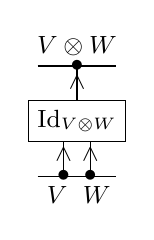
\begin{tikzpicture}[yscale = 0.7, baseline = 0pt]
\draw (0,0) -- (1,0) node[pos = 0.25,below]{\small $V$} node[pos = 0.33]{\small $\bullet$} node[pos = 0.67]{\small $\bullet$} node[pos = 0.75,below]{\small $W$};
\draw (0,2) -- (1,2) node[pos = 0.5]{\small $\bullet$} node[midway,above]{\small $V \otimes W$};
\draw (0.33,0) -- ++(0,1) node[pos = 0.4, sloped]{\footnotesize $>$};
\draw (0.67,0) -- ++(0,1) node[pos = 0.4, sloped]{\footnotesize $>$};
\draw (0.5,1) -- ++(0,1) node[pos = 0.7, sloped]{\footnotesize $>$};
\node[draw, rectangle, fill=white] at (0.5,1) {\small ${\rm Id}_{V \otimes W}$};
\end{tikzpicture}
$$
\end{Remark}

\begin{Remark}[{\cite[Remark 1.7]{Cooke}}]\label{Skmonoidal}
For a general surface $\Sigma$, the categories defined above are not monoidal because there is no notion of horizontal juxtaposition, which we used in $\mathbb{R}^2$. However, if $A = C \times [0,1]$ for a 1-manifold $C$, the category ${\rm Sk}_\mathcal{V}(A)$ is monoidal with tensor product induced by $A \sqcup A \overset{[0,\frac{1}{3}]\sqcup[\frac{2}{3},1]}\hookrightarrow A$.
\end{Remark}

\begin{Remark}[{\cite[Remarks 1.6 and 1.18]{Cooke}}]\label{rmkFunctEmbIsotOfSkCat} An orientation-preserving smooth embedding $f\colon\Sigma_1 \allowbreak\to \Sigma_2$ induces a functor ${\rm Sk}_\mathcal{V}(f)\colon{\rm Sk}_\mathcal{V}(\Sigma_1)\to {\rm Sk}_\mathcal{V}(\Sigma_2)$. It maps an object $s$, which is a bunch of coloured points in $\Sigma_1$, to $f(s)$, and a ribbon graph $T \subseteq \Sigma_1 \times [0,1]$ to $(f\times {\rm Id})(T)$. This defines a symmetric monoidal functor ${\rm Sk}_\mathcal{V}\colon ({\rm Mfld}_2^{\rm or},\sqcup) \to ({\rm Cat}_k,\otimes_k)$.

An isotopy of smooth embeddings $\lambda \colon \Sigma_1 \times [0,1] \to \Sigma_2$ between $f=\lambda_0$ and $g=\lambda_1$ induces a~natural isomorphism ${\rm rib}_\lambda\colon {\rm Sk}_\mathcal{V}(f) \Rightarrow {\rm Sk}_\mathcal{V}(g)$, where ${\rm rib}_{\lambda,s}\colon f(s) \to g(s)$ is the braid in $\Sigma_2 \times [0,1]$ drawn by $\{(\lambda_t(s),t), t \in [0,1]\}$. Homotopic isotopies give isotopic ribbon graphs, and this extends to a symmetric monoidal $\infty$-functor ${\rm Sk}_\mathcal{V}\colon ({\rm Mfld}_2^{\rm or},\sqcup) \to ({\rm Cat}_k,\otimes_k)$. It is shown in~\cite{Cooke} that this functor is the factorisation homology with coefficients in $\mathcal{V}$.
\end{Remark}

\begin{Proposition}[{\cite[Section~1.3]{Cooke}}]\label{Skmodcat}
For $C\subset \partial \Sigma$ a boundary component $($actually, a thick left boundary component, i.e., equipped with an embedding $C \times [0,2) \hookrightarrow \Sigma)$ the category ${\rm Sk}_\mathcal{V}(\Sigma)$ inherits a~structure of left ${\rm Sk}_\mathcal{V}(A)$-module category, where $A = C\times [0,1]$. Namely, one has a~functor $\rhd\colon {\rm Sk}_\mathcal{V}(A) \otimes {\rm Sk}_\mathcal{V}(\Sigma) \to {\rm Sk}_\mathcal{V}(\Sigma)$ compatible with the monoidal structure of ${\rm Sk}_\mathcal{V}(A)$. It is given by pushing points or ribbon graphs in $A$ inside $\Sigma$.
Similarly, a thick right boundary component $C\times (-1,1]\hookrightarrow \Sigma$ induces a right ${\rm Sk}_\mathcal{V}(A)$-module structure on ${\rm Sk}_\mathcal{V}(\Sigma)$.
\end{Proposition}
